%\section{Flooding and Routing Mechanisms over Wireless Ad Hoc Networks}
\section{Flooding and Routing in Spontaneous Wireless Networks}
\label{s:flood_rtg}

% Note: At some point it should be clear that we are assuming a SINGLE wireless interface per router.
% Note: Provide consistent notation message/packet throughout the chapter.

As described in section \ref{s:comm_wless}, there are important differences in the way that spontaneous wireless networks enable communication between nodes, with respect to the classic fixed/wired networks. These differences have a significant impact in the mechanisms and protocols used in wireless multi-hop scenarios to disseminate information through the network ({\em flooding}) and find and maintain paths between pairs of computers in the network ({\em routing}). This section examines several mechanisms that are used in different routing protocols, discusses the issues and problems that these mechanisms have when operating in spontaneous wireless networks, and describes some techniques to fix or overcome these issues. 

Section \ref{ss:nd} explores the use of neighbor discovery procedures in spontaneous wireless networks. Section \ref{ss:flood} describes techniques to perform efficient flooding over such networks. Finally, section \ref{ss:metrics} presents the problem of estimating link costs and using them to to identify ``good routes" over the network.  

\subsection{Neighborhood Discovery}
\label{ss:nd}

In many routing and flooding protocols, routers need to be aware of their own neighborhood. This is particularly important (although not only) in spontaneous wireless networks, in which the neighborhood may change frequently during network operation. Routers acquire knowledge about their neighborhood by way of a {\bf neighborhood discovery} mechanism.

\begin{definition}[Neighborhood Discovery]
(ND) is the process whereby each router advertises all the routers to which direct communication is possible ({\em i.e.}, the routers to which there are network links) about its presence in the network. This way, routers receiving such advertisements from other (neighboring) routers gain insight on their own neighborhood.
\end{definition}

%\begin{remark}
%About "neighbor".
%Messages in which a router advertises its presence to directly-reachable routers are typically denominated {\bf Hello messages}.
%\end{remark}

\paragraph{1-hop and 2-hop neighborhood}

Depending on the information advertised by ND messages, receiving routers learn different aspects about their neighborhood. If messages only advertise the presence of the originating router, the receiving router will acquire information about the routers that maintain links to itself. If links are bi-directional (as IP links in standard IP networks), this is sufficient for enabling bi-directional communication between routers: a router receiving a ND message from a neighbor can exchange packets in both directions with it. This is the case of traditional neighbor discovery protocols for Internet, such as the \textit{Neighbor Discovery Protocol} (NDP) for IPv6 \cite{rfc4861}, which assumes that all the links are bi-directional and is used to actively keep track of which neighbors are reachable. \ \\ \ \\
%
%Neighborhood discovery is the process whereby each router discovers the routers which are in direct communication range of itself (1-hop neighbors), and detects with which of these it can establish bi-directional communication. For traditional neighbor discovery protocol for Internet, such as \textit{Neighbor Discovery in IPv6} \cite{rfc4861}, assumes that all the links are bi-directional, and is used to actively keep track of which neighbors are reachable. 
%
In spontaneous wireless networks, bi-directional communication availability cannot be inferred from the reception of an ND advertisement, given the fact that asymmetric links are possible (section \ref{ss:issues}). This is taken into account in ND protocols for spontaneous wireless networks. In these protocols, ND advertisements (typically denominated {\bf Hello messages}), contain not only the id of the originating router, but also the list of its current neighbors ({\em i.e.}, routers from which the originating router has received Hello messages). This enables every router in the network to detect the (1-hop) neighbors with which bi-directional communication is possible, and identify the routers that belong to its 2-hop neighborhood -- that is, the set of routers that are 2-hop neighbors or ``neighbors of its neighbors''. 

\begin{itemize}
\item {\bf Example} Assume that router $A$ receives a Hello from a neighbor $B$, in which $B$ indicates to have recently received a Hello from $A$; then $A$ learns that link $A$-$B$ is symmetric. As $B$ lists identifiers of all its 1-hop neighbors in its Hello, $A$ learns its 2-hop neighbors through this process.
\end{itemize}

Together with 1-hop neighbors, additional information may be included in Hello messages -- in particular, the cost of the links towards the listed neighbors, when metrics other than hop-count (see section \ref{ss:metrics}) is used. Exchange of Hello messages is typically done periodically, although some events may trigger non-periodic Hellos ({\em e.g.}, changes in the topology). \ \\ \ \\ %({\em e.g.} ETX \cite{etx}, based on the number of expected transmissions to send successfully a packet over a link, or EDR \cite{edr}, that estimates the data rate at which packets can be sent) is used.
%
The {\em Mobile Ad Hoc Network Neighborhood Discovery Protocol} (NHDP, RFC 6130) \cite{NHDP-RFC6130} is the main ND protocol for spontaneous wireless networks. It is used as auxiliary protocol by other routing protocols that need neighborhood information to take their decisions, such as OLSRv2 (see section \ref{sec:olsr}). In NHDP, Hello messages are exchanged periodically and they contain the id of the originating router and the list of its 1-hop neighbors. The IETF also standardized an optimization of NDP for IPv6 over Low-Power Wireless Personal Area Networks (6LoWPANs). This optimization, specified in RFC 6775, adapts the operation of NDP to the lossy conditions of communications and the low-power device constraints of LoWPANs. This is done, for instance, by avoiding unsollicited messages (such as periodic router announcements), reducing the use of multicast for address resolution, limiting the duplicate address detection checks, or enabling better compression algorithms \cite{rfc6775}. \ \\ \ \\
%
%lossy, low-power, low-bit-rate, short-range; with many nodes saving energy with long sleep periods. Multicast as used in IPv6 Neighbor Discovery (ND) [RFC4861] is not desirable in such a wireless low-power and lossy network. Moreover, LoWPAN links are asymmetric and non-transitive in nature. 
%
Other routing protocols include their own Hello mechanism. This is the case of AODV \cite{AODV-RFC3561} (see section \ref{ss:aodv}) or OSPF and its MANET extensions \cite{rfc5449,rfc5614,rfc5820} (see section \ref{ss:ospfmanet}). In the last case, some approches have been explored in order to avoid redundant notifications and hence reduce control traffic by only reporting changes in the neighborhood occurred since the last Hello transmission: this principle leads to the {\em incremental Hellos} mechanism used in the Overlapping Relays extension of OSPF (OR/SP \cite{rfc5820}) and the {\em differential Hellos} mechanism used in the MANET Designated Routers extension of OSPF (OSPF-MDR \cite{rfc5614}). However, experiments show that the potential benefits (mostly, saved amount of traffic) of these two mechanisms are not significant, in particular when compared with the additional complexity they introduce in the corresponding protocols \cite{aircc}.

%\paragraph{ND Protocols and Optimizations for Wireless Multi-Hop Ad hoc Networks}

%The Mobile Ad Hoc Network Neighborhood Discovery Protocol (NHDP) \cite{NHDP-RFC6130} is the main ND protocol for wireless multi-hop ad hoc networks. It is used as auxiliary protocol by other routing protocols that need neighborhood information to take their decisions, such as OLSRv2. In NHDP, periodic Hello messages are exchanged locally so that each router can determine its 1-hop and symmetric 2-hop neighbors. The Hello message carries identifier of the originator, and its 1-hop neighbor information. Through Hello message exchanges, the router can determine the status of the link -- and in particular, detect whether bi-directional communication is possible: assume that router $A$ receives a Hello from a neighbor $B$, in which $B$ indicates to have recently received a Hello from $A$; then $A$ learns that link $A$-$B$ is symmetric. As $B$ lists identifiers of all its 1-hop neighbors in its Hello, $A$ learns its 2-hop neighbors through this process.

%Other routing protocols include their own Hello mechanism. This is the case of AODV \cite{AODV-RFC3561} (see section \ref{ss:aodv}) or OSPF and its MANET extensions \cite{rfc5449,rfc5614,rfc5820} (see section \ref{ss:ospfmanet}). In the last case, some optimizations have been explored in order to avoid redundant notifications by only reporting changes in the neighborhood occurred since the last Hello transmission: this principle leads to the  {\em incremental Hellos} mechanism used in the Overlapping Relays extension of OSPF (OR/SP \cite{rfc5820}) and the {\em differential Hellos} mechanism used in the MANET Designated Routers extension of OSPF (OSPF-MDR \cite{rfc5614}). However, experiments show that the potential benefits of these two mechanisms are not very relevant, in particular when compared with the additional complexity they introduce in the corresponding protocols \cite{aircc}.

 %Each router sends Hellos, listing the identifiers of all the routers from which it has recently received a Hello, as well as the ``status'' of the link (heard, verified bi-directional). 

%The purpose of the Hello message is to broadcast the local node topology information to the one-hop neighbors to serve the task such as link sensing and neighbor detection.

\subsection{Flooding}
\label{ss:flood}
%
Flooding is the process through which information originated in one router is disseminated across the network, so that it can be received by every other router in the network. \ \\ \ \\
%
The most obvious procedure to perform flooding from a router in a conventional IP network consists of the {\bf pure flooding} procedure:

\begin{enumerate}
\item The source router sends the message through all its network interfaces.
\item Every router that receives the message {\em for the first time} retransmits it over all the network interfaces {\em except the one over which it was received}.
\end{enumerate}

The fact that each router retransmits only {\em once} ensures that the process terminates in a finite number of steps. The fact that {\em all} routers receiving the message retransmit it ensures that the message is received --if there are no packet losses-- by every router in the network at least once. \ \\ \ \\
%
In a spontaneous wireless network, as routers communicate with {\em all} their wireless neighbors by way of a {\em single} wireless interface (see section \ref{s:comm_wless}), the straightforward usage of this mechanism implies that the source router broadcasts the message to be flooded and the neighboring routers rebroadcast it over the same interface it was received. It is known \cite{broadcaststorm} that such a naive approach is not efficient and does not scale in a wireless multi-hop scenario. Three reasons can be highlighted: 

\begin{enumerate}[a)]
\item excessive retransmissions that reduce the available bandwidth, 
\item systematic packet collisions due to concurrent transmissions of wireless interfaces (partly) sharing the same wireless channel, and 
\item duplicate packets reception due to the fact that the packet is received and retransmitted over the same interface (and, therefore, transmitted twice in the intersection between the coverage area of the sender and the receiver interface). 
\end{enumerate}

\begin{remark}
Although the three effects are closely inter-related, and all are due to the bandwidth scarcity and the semi-broadcast properties of wireless communication detailed in section \ref{s:comm_wless}, it is important to point out that they constitute {\em different} effects; solving one of them does not necessarily solve the others. 
\end{remark}

\paragraph{Excessive Number of Retransmissions and Efficient Flooding}

In a spontaneous wireless network, a single transmission from a wireless interface is received by the wireless interfaces of all the neighbors within its coverage area. If all routers retransmit the same message as they receive it, this is likely to cause a significant number of {\em redundant transmissions} -- {\em i.e.}, transmissions that do not bring new information for {\em any} of the interfaces receiving them. \ \\ \ \\
%
Consider the situation in Figure \ref{f:excessive}, in which node $A$ (in the center) floods a message to all its neighbors, and they in turn retransmit the same message so that it is received by all the 2-hop neighbors of $A$. In theory, every 2-hop neighbor has received the message -- possibly several times. The redundant retransmissions do not bring new information, but increase the probability of collisions. This effect becomes more relevant in a context of bandwidth scarcity and high network router density. %, as node $C_2$ which receives it from $B_1$, $B_2$ and $B_3$. Some retransmissions of $A$'s 1-hop neighbors are {\em redundant}, for instance $B_2$: if $B_2$ had not retransmitted the message, all the 2-hop neighbors that received $B_2$'s retransmission ($C_1$, $C_2$ and $C_3$) would have received the message via $B_1$ and $B_3$. In practice, the situation is worse: as several transmissions are being performed at the same time by close nodes that share (at least partly) the same wireless channel, the probability of packet collisions is high: several 2-hop neighbors "theoretically" covered by different 1-hop neighbors may be in practice unable to receive and decode successfully the message from $A$, due to collisions between retransmitters \cite{broadcaststorm}. 

\begin{figure}[h]
\centering
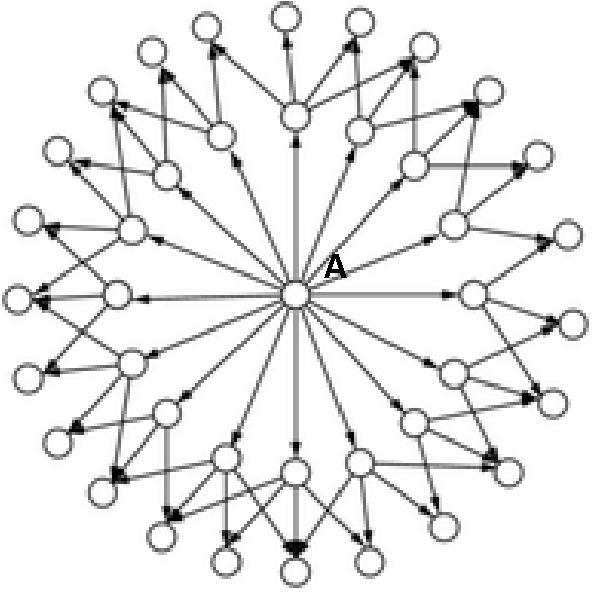
\includegraphics[width=0.4\textwidth]{Figures/purebc-crop.pdf}
\caption{Classical flooding in spontaneous wireless networks.}
\label{f:excessive}
\end{figure}

{\bf Efficient flooding} techniques explore different strategies to reduce the number of flooding retransmissions (and therefore, to decrease the amount of traffic overhead involved), while preserving as much as possible the ability of the flooding procedure to reach all (or most of) the routers in the spontaneous wireless network. \ \\ \ \\
%
For every efficient routing technique, a set of the routers that receive a message (typically, not all of them) are allowed to retransmit it. If efficient flooding reaches all routers in the network, the set of routers allowed to retransmit a message is a {\em Dominating Set} (DS) in the network graph. As only one router originates and originally sends the message, and every other forwarding router has previously received it via flooding, the set of routers and the wireless links between them usually form a {\bf Connected Dominating Set} (CDS). Given a graph $G=(V,E)$ representing a spontaneous wireless network, where $V$ is the set of vertices (representing network routers) and $E$ is the set of edges (representing network links), a Connected Dominating Set of $G$ is a subset of vertices $D \subseteq V$ with two properties:

%, assuming that the message is originally sent by only one router and every other forwarding router has received the message previously

\begin{enumerate}
\item {\em Connection}. $D$ induces a connected subgraph of $G$, that is, any node in $D$ can reach any other node in $D$ by a path that stays entirely within $D$. 
	\begin{align*}
	\forall x, y \in V &,& \exists p=(x, p_1, p_2, ..., p_n, y) \subseteq D \wedge \bar{xp_1}, \bar{p_1p_2}, ..., \bar{p_ny} \in E
	\end{align*}
\item {\em Domination}. $D$ is a dominating set of $G$, meaning that every vertex in $G$ either belongs to $D$ or is adjacent to a vertex in $D$.
	\begin{align*} 
	\forall v \in V &,& v \in D \vee ( \exists w \in D : \bar{uw} \in E )
	\end{align*}
\end{enumerate} 

%The rules used for determining which routers are selected as {\em flooding relays} lead to different techniques \cite{broadcaststorm}.

Figure \ref{f:ex_cds} displays an example of Connected Dominating Set over a network graph.

\begin{figure}[htb]	% H-must be here or [htb]
\centering
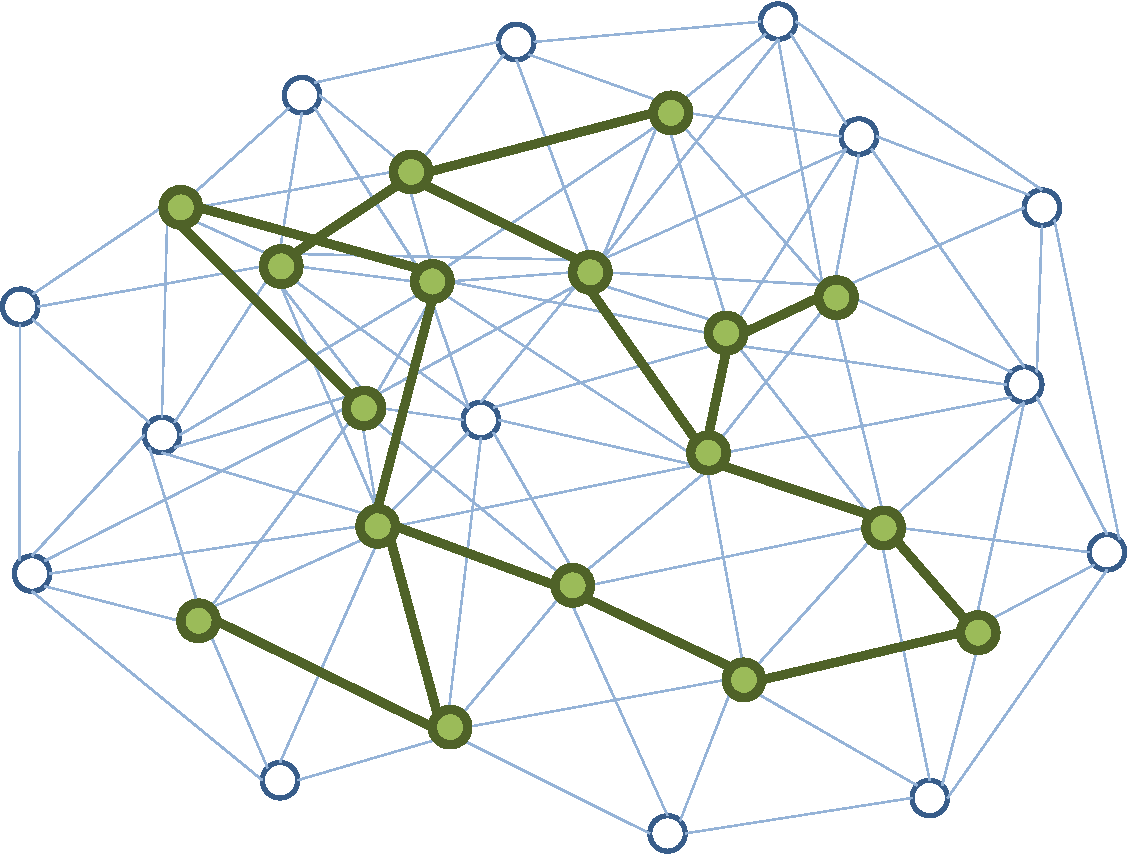
\includegraphics[width=0.6\textwidth]{Figures/excds-crop.pdf} %	** if .eps or .pdf, don't need extension}
\caption{Example of CDS (thick edges) over a network graph of 30 nodes (light edges represent communication between nodes).}
\label{f:ex_cds}
\end{figure}

The notion of CDS is useful for efficient flooding purposes: several efficient flooding techniques rely on the construction and maintenance of Connected Dominating Sets of forwarding nodes, over which packets are flooded through the network. One of the main techniques based on this principle is the {\em Multi-Point Relaying} (MPR) technique.

\begin{itemize}
\item {\bf Multi-Point Relays} \cite{mpr-hicss2002} is an algorithm through which a node selects a subset of its 1-hop neighbors (\emph{multi-point relays}) such that each 2-hop neighbor is reachable through (at least) one of the selected 1-hop neighbors ({\em MPR coverage criterion}). MPR selection requires that the selecting node knows the 2-hop neighbors that will be covered by its MPRs. By using MPR, the retransmission of flooding traffic can be significantly reduced, as shown in Figure \ref{f:mpr}, compared to classical flooding in Figure \ref{f:excessive}. 

\begin{figure}[h]
\centering
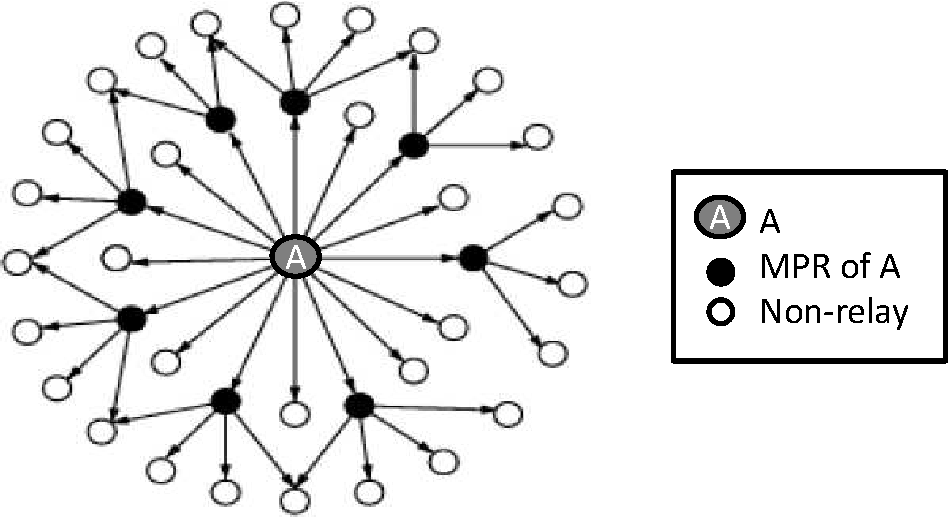
\includegraphics[width=0.65\textwidth]{Figures/mpr-crop.pdf}
\caption{Efficient flooding with Multi-Point Relays.}
\label{f:mpr}
\end{figure}

	\begin{remark}
	Note that the MPR coverage criterion does not guarantee by itself that the set of nodes selected as MPRs form a Connected Dominating Set \cite{softcom10}. The set of MPRs is by definition a dominating set, as every node is either a MPR for a neighbor, or is adjacent to its own MPR. As the heuristic for MPR selection is relative to the source, however, the subgraph resulting from MPRs and the MPR links (links connecting nodes with their relays) between them {\em is not necessarily connected}. This can be easily fixed by adding an arbitrary router and all its links to the subgraph, as proved in Cordero (2010) \cite{softcom10}.
	\end{remark}

%\begin{itemize}
%\item We present MPR: MPR, by which each router is able to, efficiently, conduct network-wide broadcasts. Each router designates, from among its bi-directional neighbors, a subset (MPR set) such that a message transmitted by the router and relayed by the MPR set is received by all its 2-hop neighbors
%\end{itemize}

Multipoint relays of a router can be used to perform efficient flooding, but the principle can be used for performing other networking operations. The MPR selection algorithm can be slightly modified so that the overlay that includes all links between routers and its (modified) multi-point relays is sufficient to compute shortest paths over the underlying network \cite{softcom10}. This result has been exploited in some extensions of OSPF for MANETs, as shown in section \ref{s:wospf}.

\end{itemize}

%The idea behind different kind of efficient flooding techniques is to find a reduced CDS. One of these techniques is the {\bf Multi-Point Relaying} (MPR) technique.


\paragraph{Systematic Packet Collisions and Jittering Techniques}

Consider the spontaneous wireless network of Figure \ref{f:syspcol}, in which router $A$ floods a message through the network. The broadcast transmission of $A$ is received at the same time by $B$ and $C$, which retransmit the message towards $E$ and $D$ (in the case of $B$) and $D$ and $F$ (in the case of $C$). Then, concurrent retransmissions from $B$ and $C$ cause a systematic packet collision from $D$'s perspective.

\begin{remark}
In this example, the collision could not be detected with any CSMA\footnote{Carrier Sense Multiple Access. CSMA is a medium access control (MAC) protocol for wireless networks in which nodes sense the medium before transmitting, and only transmit if the sensed medium is idle, that is, if the node does not detect any ongoing transmission within its reception range. See {\em e.g.} Tanenbaum {\em et al.} \cite{tanenbaum} for reference.} layer 2 mechanism neither by $B$ nor by $E$, due to the fact that $B$ and $E$ are not neighbors to each other. $B$ is a {\em hidden node} for $E$ (and vice versa).
\end{remark}

\begin{remark}
Note that this problem cannot be addressed only by way of {\em efficient flooding} approaches: none of the retransmissions by $B$ and $E$ are redundant, so none of them could be avoided without leaving nodes uncovered ($C$ if $B$ does not retransmit, $F$ if $E$ does not retransmit). 
\end{remark}

\begin{figure}
\centering
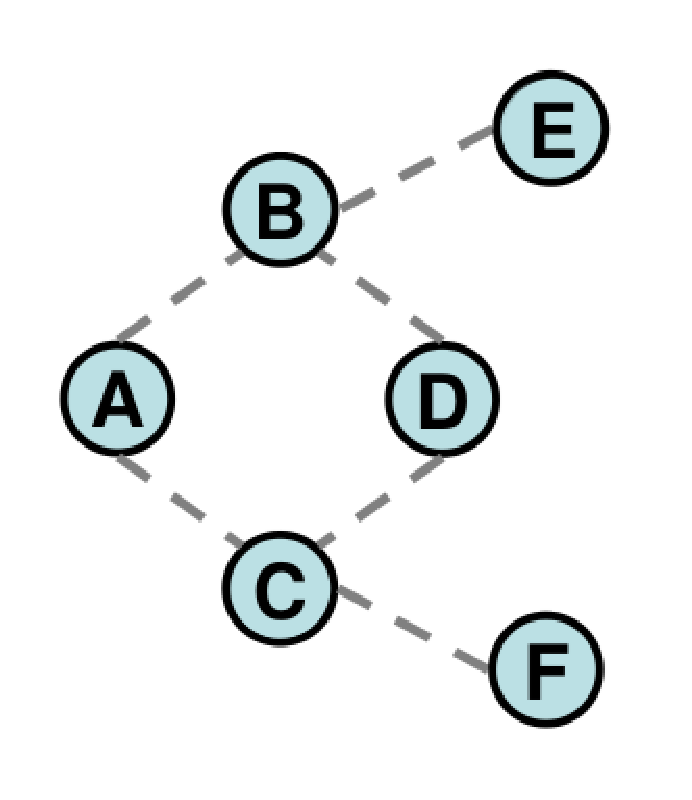
\includegraphics[width=0.2\textwidth]{Figures/abcdef-crop.pdf}
\caption{An example of spontaneous wireless network. {\em (Broken lines denote direct communication)}}
\label{f:syspcol}
\end{figure}

The fact that flooded messages are forwarded simultaneously by wireless interfaces receiving them through the same wireless shared medium may cause packet collisions during the flooding procedure (depending on the network topology at the time of flooding). Unlike other packet transmissions for which the collision probability may vary depending on the traffic pattern, these flooding collisions are {\em systematic} and will occur, for a given network topology and flooding algorithm, any time that the source node floods a new message (in the example, any time $A$ floods a message). \ \\ \ \\
%
This effect could be alleviated by allowing routers to wait a random amount of time (denominated {\bf jitter}) before retrasmitting a flooded message, in order to reduce the probability of concurrent transmissions by neighboring wireless interfaces. This technique is known as {\bf jittering}, and has been standardized by the IETF in RFC 5148 \cite{jitter-RFC5148}. The recommendation from RFC 5148 is that delays are selected following an uniform distribution between $0$ and a maximum jitter value, $MAX\_JITTER$. Figure \ref{f:jitter} illustrates the effect of jittering techniques in the network example of Figure \ref{f:syspcol}. In the example, node \textit{A} is flooding a packet to all the other nodes. When node \textit{B} and \textit{C} receive the packet from \textit{A}, instead of retransmitting the packet immediately, they wait a random delay. In this way, simultaneous transmission of $B$ and $C$ (which can cause collision at $D$ in this case) can be avoided. \ \\ \ \\
%
\begin{figure}[htb]
\centering
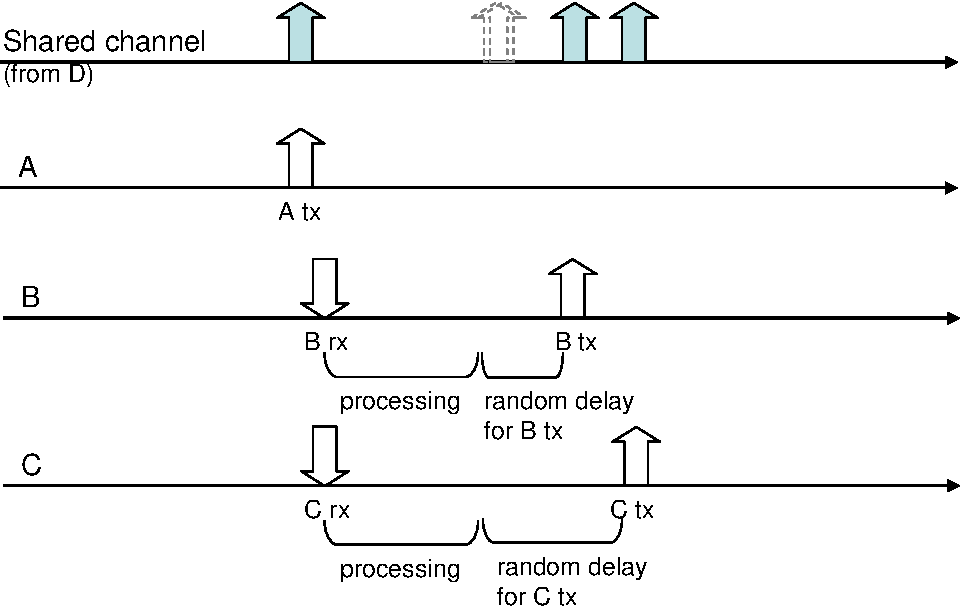
\includegraphics[width=0.6\textwidth]{Figures/jitter4flooding-crop.pdf}
\caption{Use of jitter for flooding. Node \textit{A} is flooding a packet in a network. Node \textit{B} and \textit{C} wait a random delay before the packet is retransmitted. The dashed overlapping arrows represent the packet collision that would occur if no jitter were used.}
\label{f:jitter}
\end{figure}
%
Although jittering can be theorically implemented at different layers of the protocol stack, it has been shown that its use in layers upper than L3 brings little benefit \cite{jitter-broadcast}. As the problem of systematic collisions affects every L3 routing protocol using wireless flooding, jittering techniques can be implemented by different protocols. The addition of random delays in flooded packets impacts differently in proactive and reactive protocols, given the different use of flooding in both routing strategies. Other jittering effects are due to the specifities of the techniques employed in each case. In proactive protocols where jitter is used (as described in RFC 5148 \cite{jitter-RFC5148}, which recommends to introduce random delays and piggyback all pending messages when a transmission is scheduled), such as OLSR or the OSPF extensions for MANETs, jittering leads to longer LSA messages -- this may cause additional packet collisions, if jitter values are not configured properly \cite{INFOCOM-jitter,jitter-wpc}. In reactive protocols such as AODV, where jitter is used for Route Request (RREQ) flooding, the addition of random delays may lead to suboptimal path selections, which can be minimized by adapting the random distribution used for determining jitter values \cite{Infocom12, wiopt}.  

\paragraph{Duplicate Packets and Detection Techniques}

The reception of duplicate packets is a common situation in wireless flooding, due to the fact that flooded messages are retransmitted by forwarding nodes over the same wireless interface in which they were received. Consider the situation of Figure \ref{f:dpd}: router \textit{N2} is retransmitting a broadcast packet received from router \textit{N1} on the same interface as the one over which it was received, so as to ensure receipt also by router \textit{N3}, causing router \textit{N1} to receive the packet a second time.

\begin{figure}[ht]
\centering
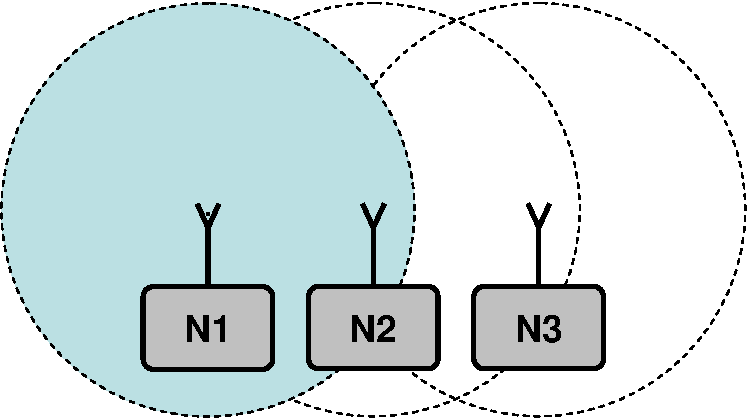
\includegraphics[width=0.4\textwidth]{Figures/dpd.pdf}
\caption{The need for duplicate detection: retransmission over the same interface as a packet was received.}
\label{f:dpd}
\end{figure}

Depending of the protocol and the use it makes of flooding and of flooded packets, the way to detect duplicate packets might be different. In link-state routing protocols such as OLSR or OSPF, for instance, flooded messages are link-state advertisements (LSAs) that are stored locally before being retransmitted, in case they bring fresh topology information; in this case, a duplicate LSA can be easily recognized by checking whether the LSA is already installed in the local Link-State Database (LSDB). If flooded messages are not stored locally, the protocol needs to store state for every forwarded message in order to detect a duplicate -- this is, for instance, the strategy of the Simplified Multicast Forwarding (SMF) protocol \cite{rfc6621}. In case a received message was already received and forwarded, it is dropped.

%\subsection{Synchronization}
\subsection{Link Metrics}
\label{ss:metrics}

\glslink{metric}{Metrics} are used to evaluate the cost of a link or a path (set of links), so that a routing protocol is able to determine whether a path or a link should be preferred over another. \ \\ \ \\
%
The simplest link \glslink{metric}{metric} is the {\bf hop-count}: a link has \glslink{metric}{metric} 1 if it is available, 0 otherwise. Typically, in the early versions of routing protocols for spontaneous wireless networks (e.g., AODV, OLSRv1 for mobile ad hoc networks), only the hop-count \glslink{metric}{metric} is used. This way, the \glslink{metric}{metric} or cost for a path is equal to the number of hops involved. \ \\ \ \\
%
When a route between two hosts is being calculated under the hop-count metric, paths with less number of hops are preferred to paths with more number of hops. However, using only minimum hop routes in spontaneous wireless networks may result in suboptimal routing in practice, as the minimum-hop routes are not necessarily the best ones \cite{couto03, wang95}. \ \\ \ \\
%
Figure \ref{f:metric} give an example showing the limit of hop-count metric. The minimum hop route from node \textit{A} to \textit{B} is $\{A,X,B\}$. However, the links $\bar{AX}$ and $\bar{XB}$ are poor with high loss rate (but still able to deliver packets), and $\bar{AY}$, $\bar{YZ}$, $\bar{ZB}$ are reliable links. In this case, $\{A,Y,Z,B\}$ is preferred to the route with minimum hop count. \ \\ \ \\
%
\begin{figure}
\centering
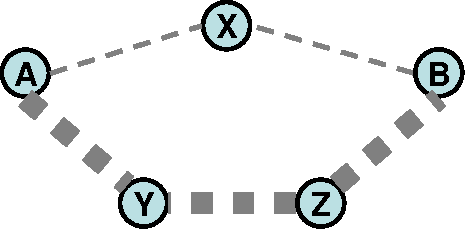
\includegraphics[width=0.25\textwidth]{Figures/axb-crop.pdf}
\caption{An example of different link metric. $\bar{AX}$, $\bar{XB}$ are unreliable links; $\bar{AY}$, $\bar{YZ}$, $\bar{ZB}$ are reliable links.}
\label{f:metric}
\end{figure}
%
Because of the limitation of hop-count metric, new metrics need to be defined. The link metrics used in spontaneous wireless network are expected to have following properties \cite{metrics}:

\begin{itemize}
\item {\bf Dimensionless}. The \glslink{metric}{metric} may correspond to specific physical information, but this knowledge is not used by the routing protocol. 
\item {\bf Additiveness}. The \glslink{metric}{metric} of a route is the sum of the metrics of the links forming that route. It also requires a \glslink{metric}{metric} where a low value of a link \glslink{metric}{metric} indicates a "good" link a high value of a link \glslink{metric}{metric} indicates a ``bad" link. 
\item {\bf Directionality}. The \glslink{metric}{metric} from a router $A$ to router $B$ does not need be the same as the \glslink{metric}{metric} from $B$ to $A$. This is a direct consequence of the fact that wireless links are not bi-directional. 
\end{itemize}

The kind of \glslink{metric}{metric} used in a network depends on the link/physical layer protocol used, the type of information that is available from lower layers, the application requirements, etc. Some examples of link \glslink{metric}{metric} include delay, packet loss probability (Expected Transmission Count, ETX \cite{etx}, that estimates the average number of transmissions before success over a link), queue length (at the receiver) or data rates (Expected Data Rate, EDR \cite{edr}; this \glslink{metric}{metric} is not additive, thus a mapping that inverts its ordering must be applied).

%%\begin{itemize}
%%\item Delay. 
%%\item Packet loss probability. 
%%\item Queue length. 
%%\item Data rates. It is not additive, thus a mapping that inverts its ordering must be applied. 
%%\end{itemize}
